\chapter{Análise de Resultados} \label{ch:analise_resultados}

Este capítulo apresenta a análise dos resultados obtidos a partir do desenvolvimento da linguagem proposta, organizados com relação aos objetivos específicos estabelecidos na \autoref{sec:objetivos}. Após avaliar como cada objetivo específico foi alcançado, eles serão sintetizados para determinar se o objetivo geral do trabalho foi atingido.

\section{Implementação da Solução}

A implementação do protótipo de interpretador para a linguagem proposta se mostrou muito parecida com a implementação de interpretadores de linguagens tradicionais. Isso se deve ao fato dele possuir todas as fases genéricas de um interpretador tradicional implementadas, já que foi feito com base na primeira metade do livro \textit{Crafting Interpreters}, e consequentemente feito com base em Jlox \cite{craftinginterpreters}.

Saindo do escopo de fases de um interpretador e indo mais a fundo na implementação, também foi possível observar semelhanças de sintaxe com linguagens tradicionais. Um exemplo disso é a sintaxe de declaração de sistemas, que é muito parecida com a sintaxe de declaração de funções em Jlox, Rust, e muitas outras linguagens \cite{rustbook,craftinginterpreters}.

Usando regras de produção, a figura \ref{fig:decl_sistema_funcao} demonstra a semelhança entre a sintaxe de declaração de sistemas na linguagem proposta e a sintaxe de declaração de funções em Jlox. Nota-se que há apenas duas diferenças: a palavra-chave \texttt{system} no lugar de \texttt{fun} e a sintaxe de \textit{query} no lugar da lista de parâmetros.

\begin{figure}[H]
	\centering
	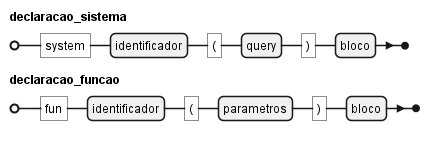
\includegraphics[width=0.45\textheight]{../diagrams/decl_sistema_funcao.png}
	\caption{Diagrama de sintaxe comparando declaração de sistemas e de funções.}
	\fonte{Elaboração própria com PlantUML feita com base no interpretador nosso e no de Jlox \cite{craftinginterpreters}.}
	\label{fig:decl_sistema_funcao}
\end{figure}

Vale ressaltar que semelhanças como essa estão presentes em outras partes da sintaxe da linguagem proposta, e foram intencionalmente feitas para facilitar a legibilidade e a facilidade de escrita através da familiaridade com outras linguagens, conforme discutido na \autoref{sec:design_linguagem}.

Fora as semelhanças, as diferenças na implementação da linguagem proposta foram encontradas principalmente na semântica e na pragmática \cite{designconceptsinlanguages}, que foram adaptadas para suportar os conceitos de ECS.

Ainda no exemplo de declaração de sistemas, a semântica foi feita de forma que o interpretador reconheça um sistema como uma função que atua sobre entidades e seus componentes de forma automática. Já a pragmática foi feita através da ligação da sua sintaxe com a API da biblioteca de ECS Flecs.

A fim de melhor documentar o processo de desenvolvimento da implementação, a seção seguinte detalha as decisões tomadas e os desafios encontrados durante o desenvolvimento do interpretador de forma exaustiva.

\section{Decisões Tomadas e Desafios Encontrados}

\section{Viabilidade e Limitações da Solução}
